\documentclass[main.tex]{subfiles}

\begin{document}
\sloppy

\vspace{1.0cm}

\section{Reimplementazione dell'interpolazione}\label{sec:Interpolation}
\lstset{language=UEcpp}
L'oggetto interpolazione si occupa di emulare lo spostamento di un vero motore nella realtà. Ad una interpolazione è possibile impostare un target ed il valore fornito in output da questo oggetto verrà modificato ad ogni tick seguendo una velocità che accelera, rimane costante e decelera, fino a raggiungere il suddetto target.

L'ogetto interpolazione originale era implementato attraverso varie formule matematiche di derivate e integrali, che però erano difficile da modificare se necessario, non erano documentate, ma soprattutto non funzionavano: Come già spiegato nell'introduzione, molte volte il valore dell'interpolazione non convergeva al target continuando ad alternarsi intorno ad esso, oppure era molto lento. Inoltre non era possibile specificare davvero la velocità in secondi con il quale doveva accellerare o arrivare a destinazione, cosa invece richiesta da GDTF.\newline

In questo capitolo tratto come è stato completamente re-implementato l'algoritmo di interpolazione in una maniera più standard. Dopo essermi confrontato con le persone che lavorano al firmware dei fari, nel reparto R\&D di ClayPaky, ho anche avuto conferma che la mia implementazione è molto vicina a quella presente nei fari veri.

%\subsection{Problemi riscontrati}\label{subsec:4_oldProblems}
\subsection{Prima implementazione}\label{subsec:4_trafficImplementation}
Un problema simile a questo era già stato riscontrato nell'implementazione di un progetto per l'esame di \say{Metodologie di Programmazione} \cite{TrafficGame}: Il progetto consisteva in un videogioco in cui erano presenti delle macchine che dovevano muoversi senza scontrarsi con quelle davanti. Ogni macchina doveva avere un movimento realistico, quindi, partendo da ferma, doveva accelerare e, per fermarsi, doveva decelerare. Sono quindi partito da quel progetto per la scrittura di questo algoritmo. Le uniche due differenze consistono che nel progetto d'esame le macchine potevano andare solamente \say{avanti} ed il tempo tra un frame e l'altro del videogioco era constante, mentre su unreal engine è variabile. Quest'ultima differenza ci porta a dover mettere in atto numerose modifiche spiegate nei capitoli successivi.\newline

Internamente la nostra velocità è salvata come \lstinline{float currentSpeed;} che dovrà rimanere nel range [0, 1]. All'interno dell'oggetto interpolazione verranno salvati due parametri:
\begin{itemize}
    \item \lstinline{acceleration}: quanta velocità perdiamo o guadagniamo ogni secondo, espressa come valore normalizzato tra [0, 1].
    \item \lstinline{maxPhysicalSpeed}: quanta distanza fisica viene percorsa ogni secondo mentre stiamo alla velocità massima (Da qui in avanti chiamata \say{maxSpeed}).
\end{itemize}
\begin{figure}[H]
    \centering
    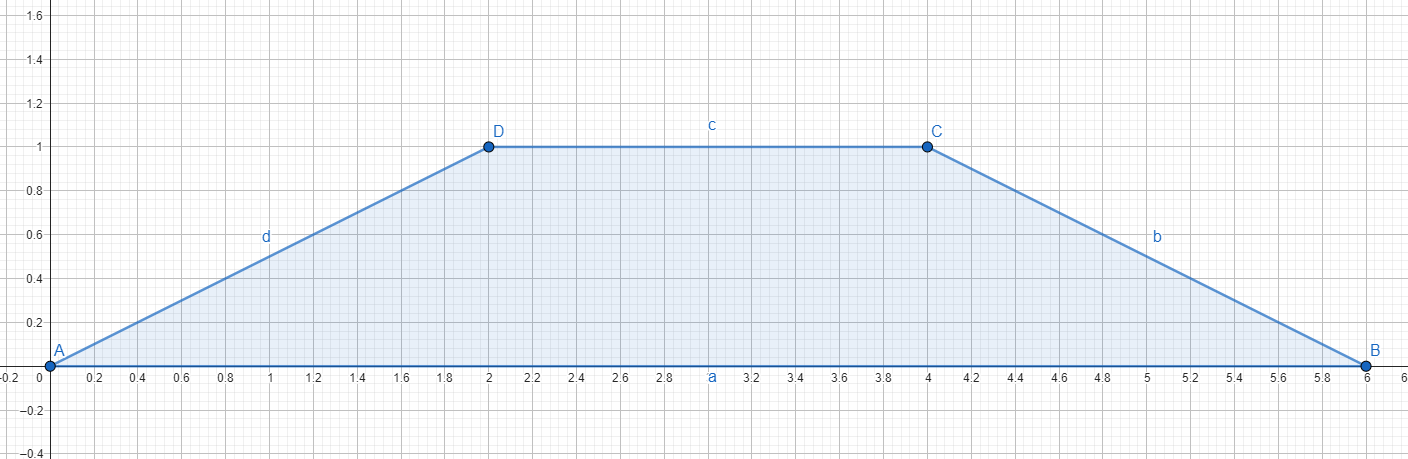
\includegraphics[width=1\linewidth]{img/interpolazione/normalSpeed.png}
    \caption{Sulle Y la nostra velocità, sulle X il tempo. Questo è un esempio normale di ciclo di accelerazione: acceleriamo fino a che non raggiungiamo maxSpeed e rimaniamo a velocità costante fino a che non deceleriamo del tutto. La distanza percorsa corrisponde all'integrale della funzione disegnata dall'andamento della velocità}
    \label{fig:4_normalSpeed}
\end{figure}

L'aggiornamento dello stato dell'interpolazione viene effettuato dentro la funzione \lstinline{Update()}, che può essere chiamata ad intervalli di tempo irregolari. Chiameremo \say{tick} oppure \say{frame} il momento in cui viene chiamata \lstinline{Update()}. Il delta tempo tra un frame e l'altro è passato come argomento ad \lstinline{Update()}

Prima di iniziare, enuncio dei concetti ricorrenti all'interno di questo capitolo:
\begin{itemize}
    \item L'interpolazione funziona in entrambi le direzioni, ma noi, all'interno della spiegazione, consideriamo solamente il caso in cui andiamo avanti (\say{FORWARD}). Se \lstinline{float currentAcceleration;} è positiva vuol dire che stiamo accelerando, altrimenti stiamo decelerando. Se la nostra direzione fosse opposta, \lstinline{currentAcceleration} e \lstinline{currentSpeed} avrebbero i segni invertiti.
    \item timeToFullyAccelerate (\say{TTFA}): È il tempo richiesto per raggiungere maxSpeed a partire da fermi e viceversa. Per ottenere quanto tempo ci mettiamo a raggiungere velocità massima o minima a partire da una velocita intermediaria, basta moltiplicare tale velocità per TTFA, poiché tutti i nostri calcoli sono nel range [0, 1] ($TimeToAccelerate = (TTFA * (1 - currentSpeed)) / 1$ e $TimeToStop = (TTFA * currentSpeed / 1)$)
    \begin{figure}[H]
        \centering
        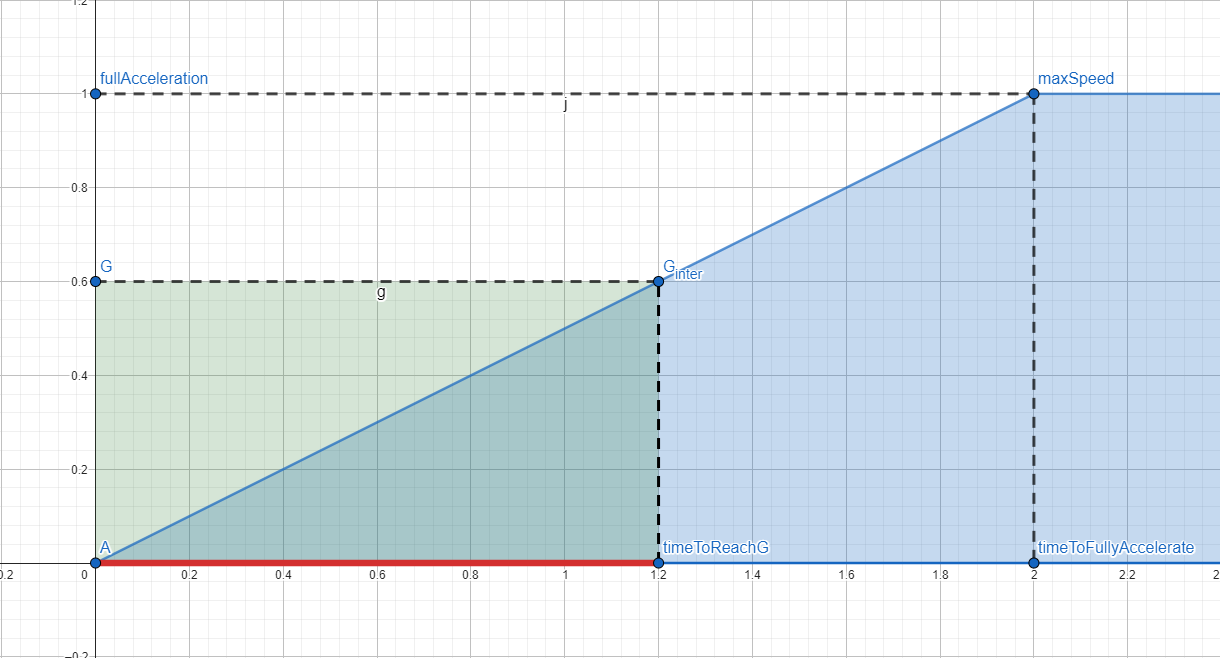
\includegraphics[width=.65\linewidth]{img/interpolazione/timeToFullyAccelerate.png}
        \label{fig:4_timeToFullyAccelerate}
    \end{figure}
    \item Convertire la velocità interna a velocità reale: Per le stesse motivazioni di sopra, basta moltiplicare la velocità interna con \lstinline{maxPhysicalSpeed}. Questo ragionamento si applica per tutto, anche per le distanze.
\end{itemize}

A questo punto, analizziamo la funzione di Update originale. Gli step saranno numerati per indicare nei capitoli successivi dove verranno aggiunte le modifiche al codice per compensare il fatto che \lstinline{Update()} venga chiamata ad intervalli irregolari.
\newcommand{\itemEnu}{\stepcounter{enumi}\textbf{(\number\numexpr\value{enumi}\relax) }}
\begin{enumerate}
    \item Controlliamo se \lstinline{CurrentValue} ha raggiunto \lstinline{TargetValue}. Se si, ritorniamo, altrimenti \itemEnu controlliamo se l'interpolazione è abilitata. Se no, impostiamo \lstinline{TargetValue = CurrentValue} e ritorniamo.
    \item Calcoliamo quanta distanza abbiamo percorso dall'ultimo tick usando \lstinline{calcNextMovement()}.
    \item Calcoliamo quanta distanza percorreremmo se iniziassimo a decelerare in questo tick, usando \lstinline{getStopDistance()}.
    \item Controlliamo se siamo fermi o meno.
    \item Se siamo fermi, controlliamo se abbiamo raggiunto TargetValue. Se si, \itemEnu terminiamo l'interpolazione. Altrimenti, \itemEnu calcoliamo la nuova direzione (\lstinline{FORWARD} o \lstinline{BACKWARD}) e \itemEnu forziamo l'inizio dell'interpolazione.\newline
    Se non siamo fermi, \itemEnu controlliamo se la distanza calcolata precedentemente è più grande della differenza tra CurrentValue e TargetValue. Se si, \itemEnu vuol dire che dobbiamo iniziare a decelerare, altrimenti sorpasseremo TargetValue.
    \item Controlliamo il nostro status, ovvero se stiamo accelerando (\lstinline{status = true}) o decelerando (\lstinline{status = false}). Se lo stato è cambiato rispetto allo scorso tick (oppure se stiamo forzando l'inizio dell'interpolazione), \itemEnu iniziamo ad accelerare o decelerare impostando, nel primo caso, \lstinline{currentAcceleration = acceleration}, altrimenti, nel secondo caso, \lstinline{currentAcceleration = -acceleration}.
    \item Controlliamo se l'interpolazione è finita testando se stiamo fermi e abbiamo raggiunto TargetValue. Se si, ritorniamo, altrimenti \itemEnu aggiungiamo a CurrentValue la distanza percorsa nel tick corrente.
\end{enumerate}

Nella funzione \lstinline{Update()} sono state chiamate altre funzioni:
\begin{itemize}
    \item \lstinline{calcNextMovement()}: Questa funzione si occupa di aggiornare la velocità corrente e calcolare la distanza percorsa tra questo frame ed il precedente. La nuova velocità è calcolata come $newSpeed += acceleration * DeltaSeconds$. Se dopo questo calcolo siamo usciti dal range [0, 1] vuol dire che tra questo tick ed il precedente ci siamo fermati del tutto oppure abbiamo raggiunto la velocità massima. In questo caso clampiamo la velocità e calcoliamo quanto tempo ci mettiamo a raggiungere il limite del range a partire dalla velocità precedente: $remainingTime = speedToRange * TTFA$. Se ci siamo fermati chiamiamo \lstinline{__calcNextMovement_internal()} con solamente il remainingTime. Se invece abbiamo raggiunto la velocità massima, chiamiamo \lstinline{__calcNextMovement_internal()} per calcolare lo spazio percorso fino a che non abbiamo raggiunto maxSpeed ed aggiorniamo DeltaSeconds come la differenza da quel momento al tick corrente $DeltaSeconds -= remainingTime$. Infine, se ci stiamo muovendo, chiamiamo \lstinline{__calcNextMovement_internal()} per calcolare ciò che resta del nostro movimento. Quest'ultima chiamata è valida sia quando non raggiungiamo i limiti della velocità e sia quando raggiungiamo maxSpeed.
    \begin{figure}[H]
        \centering
        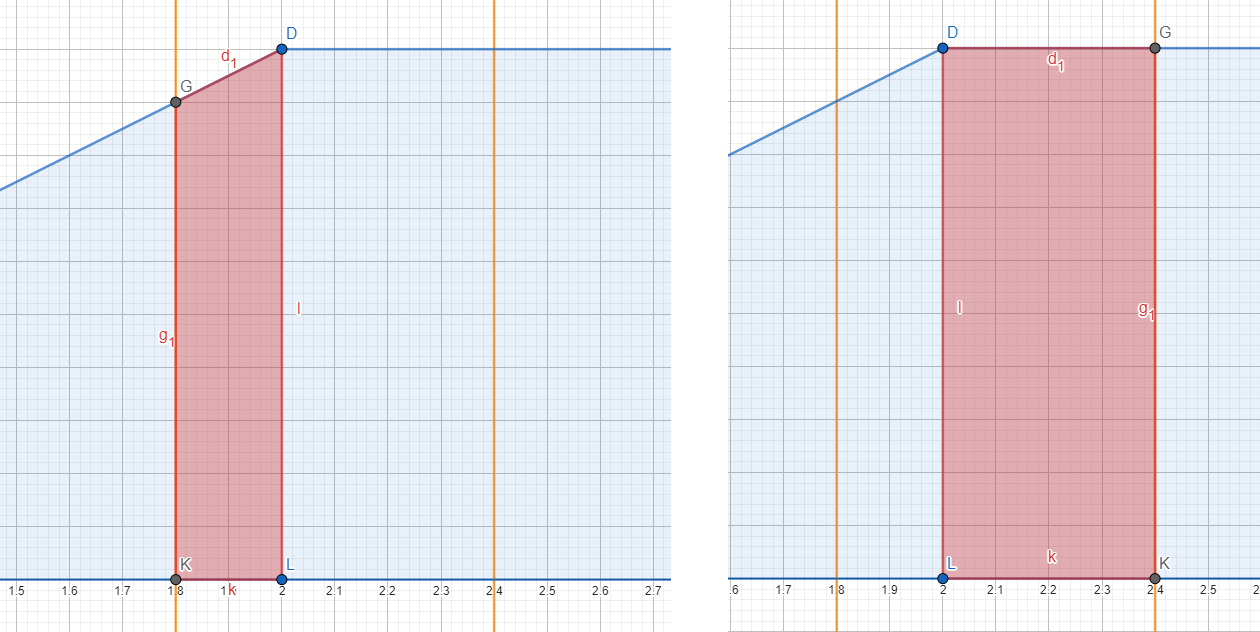
\includegraphics[width=.8\linewidth]{img/interpolazione/calcNextMovementLateCall.png}
        \caption{I due quadrilateri in cui la velocità viene divisa per calcolarne l'area}
        \label{fig:4_calcNextMovementLateCall}
    \end{figure}
    \item \lstinline{__calcNextMovement_internal()}: Questa funzione si occupa di calcolare lo spazio percorso in DeltaSeconds a partire dalla velocità precedente fino ad arrivare alla velocità corrente. Il calcolo viene effettuato scomponendo il quadrilatero in un rettangolo con un altezza pari a \lstinline{previousSpeed} a cui va sommata l'area di un triangolo che come altezza ha la differenza tra \lstinline{currentSpeed} e \lstinline{prevSpeed}. Questo calcolo funziona sia quando si accelera, che quando si è a velocità costante (il triangolo avrà area 0, poiché l'altezza sarà uguale a 0), che quando si decelera (il triangolo avrà area negativa)
    \begin{figure}[H]
        \centering
        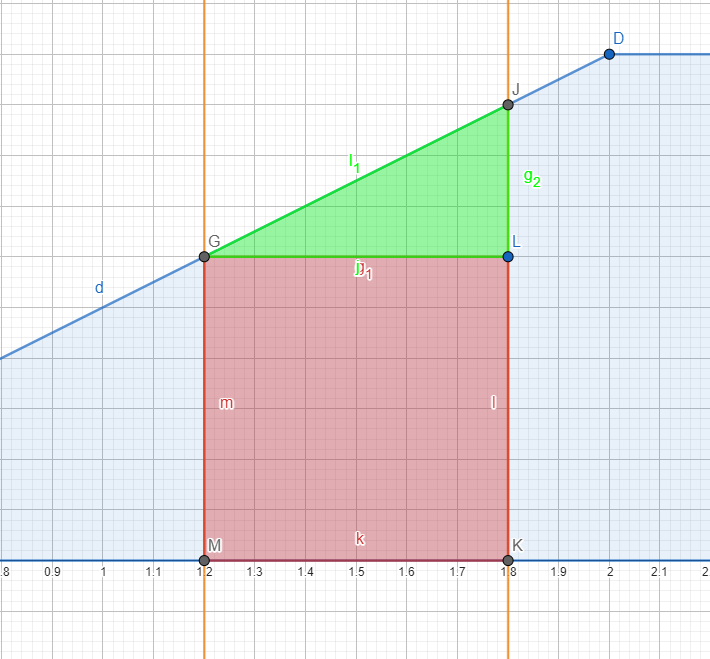
\includegraphics[width=.6\linewidth]{img/interpolazione/calcNextMovementInternalB.png}
        \caption{Scomposizione dell'area per il calcolo del movimento tra un tick e l'altro}
        \label{fig:4_calcNextMovementInternalB}
    \end{figure}
    \item \lstinline{getStopDistance()}. Questa funzione calcola il movimento percorso se iniziassimo a decelerare dal frame corrente senza poi riaccelerare. Calcola l'area di un triangolo che come altezza ha la velocità corrente e come base ha TTS (TimeToStop)
    \begin{figure}[H]
        \centering
        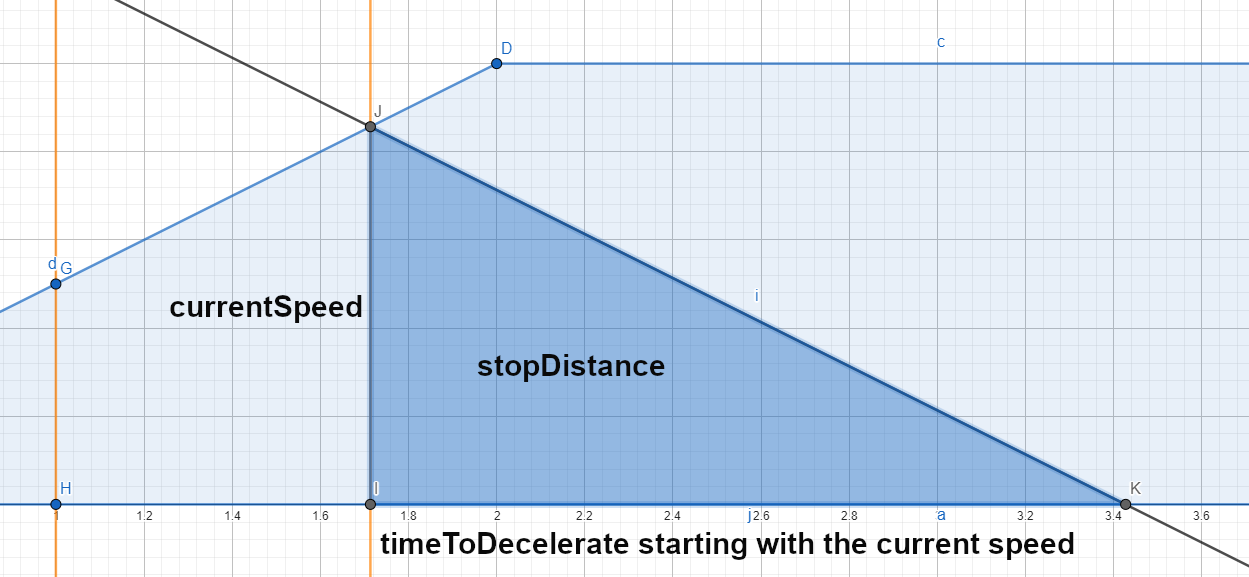
\includegraphics[width=.65\linewidth]{img/interpolazione/getStopTimeLabel.png}
        \label{fig:4_getStopTimeLabel}
    \end{figure}
\end{itemize}

\subsection{Modifiche all'implementazione}\label{subsec:4_edits}
Come scritto in precedenza, il codice scritto fin'ora funziona a patto che i DeltaSeconds tra un tick e l'altro siano costanti e ravvicinati. Questo non è il caso di UnrealEngine e, di conseguenza, bisogna aggiungere delle modifiche all'algoritmo originale per ottenere una interpolazione corretta.

\subsubsection{Compensate Late Call}\label{subsubsec:4_2_CompensateLateCall}
Quasi sempre accade che il momento esatto in cui dovremmo iniziare a decelerare si trovi tra il tick precedente e quello corrente. Iniziando a decelerare in questo tick ci ritroveremo alla fine con più distanza percorsa del dovuto, sorpassando TargetValue.
\begin{figure}[H]
    \centering
    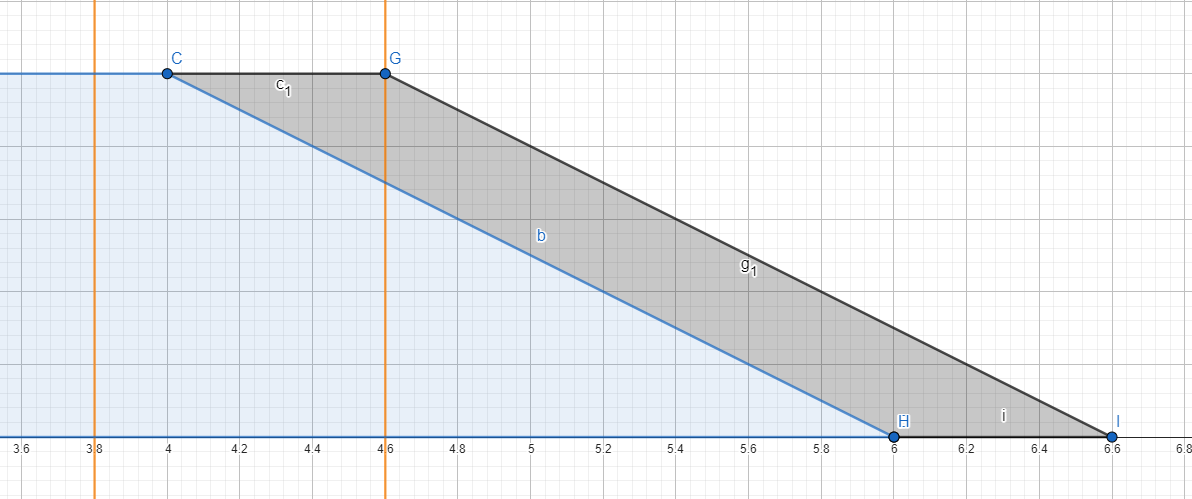
\includegraphics[width=.65\linewidth]{img/interpolazione/compensateLateCall.png}
    \caption{In grigio il movimento extra che viene erroneamente fatto}
    \label{fig:4_compensateLateCall}
\end{figure}

Questa correzione viene effettuata quando iniziamo a decelerare e se la stopDistance supera TargetValue (Chiameremo la differenza tra i due valori \say{distanceDifference}), ma non abbiamo ancora superato TargetValue. Viene effettuata tra quando viene deciso che dobbiamo iniziare a decelerare e immediatamente prima di cambiare il valore di accelerazione (Tra i punti \textbf{12} e \textbf{13} della funzione di \lstinline{Update()}). La prima cosa che fa è effettuare un rollback di qualsiasi movimento svolto durante questo frame e successivamente controlliamo se nel tick precedente stavamo accelerando, ma al tick corrente stiamo a velocità costante. Se si vuol dire che tra i due frame abbiamo raggiunto la velocità massima e dobbiamo scoprire se avremmo dovuto iniziare a decelerare prima o dopo averla raggiunta. Per eseguire questo controllo usiamo \lstinline{__calcNextMovement_internal()} per calcolarci lo spazio percorso fino a raggiungere maxSpeed e sommiamo questo valore a quello ottenuto da una chiamata a \lstinline{getStopDistance()} con velocità pari ad 1. Se questa distanza appena calcolata sommata a CurrentValue è più grande di TargetValue vuol dire che avremmo dovuto iniziare a decelerare prima di raggiungere la velocità massima, e viceversa. Nel primo caso ricalcoliamo la distanceDifference come la differenza tra la precedente somma e Target Value, nel secondo caso faremo semplicemente finta di essere a velocità costante già dal frame precedente.
\begin{figure}[H]
    \centering
    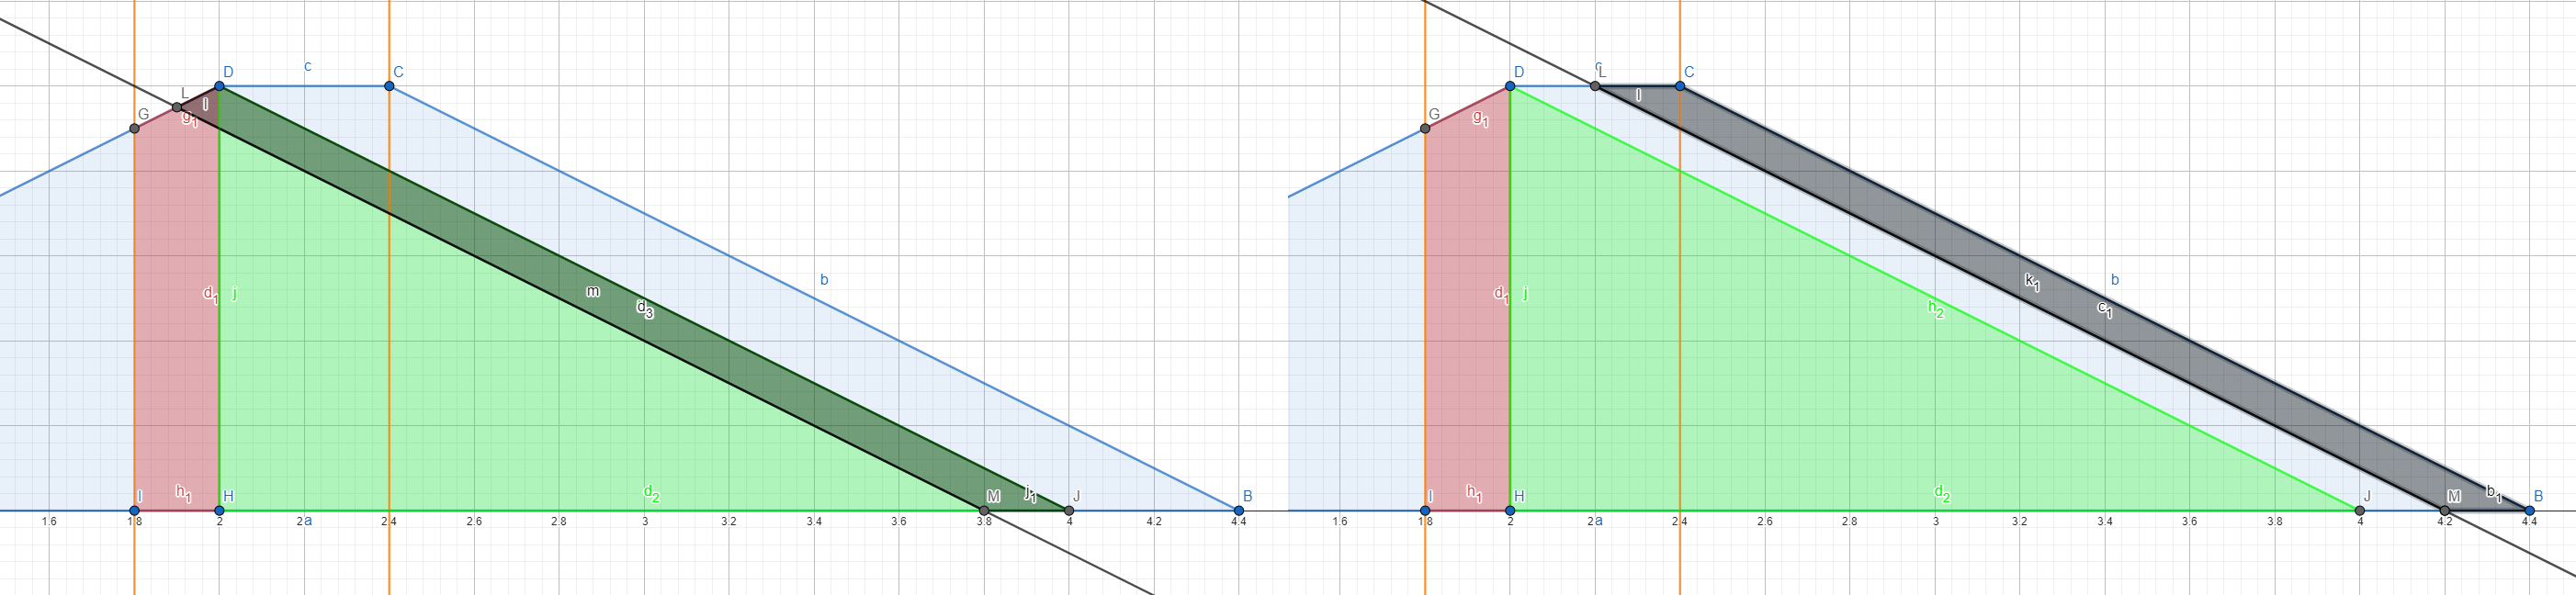
\includegraphics[width=1\linewidth]{img/interpolazione/compensateLateCall3Case.png}
    \caption{In rosso lo spazio percorso fino a raggiungere maxSpeed, in verde la stopDistance a partire da maxSpeed. La somma dei due è quella testata nei precedenti check. In grigio la differenza con TargetValue: a sinistra abbiamo il caso in cui avremmo dovuto iniziare a decelerare prima di raggiungere maxSpeed, a destra dopo}
    \label{fig:4_compensateLateCall3Case}
\end{figure}

Per calcolare il momento esatto in cui avremmo dovuto iniziare avremmo due casi possibili: 
\begin{itemize}
    \item \textbf{Siamo a velocità costante}: La differenza di spazio percorso è un parallelogramma (Vedi la seconda immagine di \ref{fig:4_compensateLateCall3Case}) di cui sappiamo l'area (distanceDifference) e l'altezza (1, ovvero maxSpeed). Possiamo calcolarci la base (ovvero la differenza tra DeltaTime ed il momento in cui avremmo dovuto iniziare a decelerare) con una semplice formula inversa: $timeDifference = distanceDifference / speed$.
    \hspace{2cm}
    
    \begin{minipage}{.45\textwidth}
        \item \textbf{Stiamo accelerando}: Poiché in questo caso stiamo trattando un poligono irregolare (Vedi figura \ref{fig:4_compensateLateCallAccel1}), non possiamo applicare direttamente formule inverese. Scomponiamo quindi tale quadrilatero in un triangolo ed un quadrato come nella figura \ref{fig:4_compensateLateCallAccel2} e mettiamo a sistema tutte le dimensioni che sappiamo di tale figura.
    \end{minipage}
    \begin{minipage}{.475\textwidth}
        \begin{figure}[H]
            \centering
            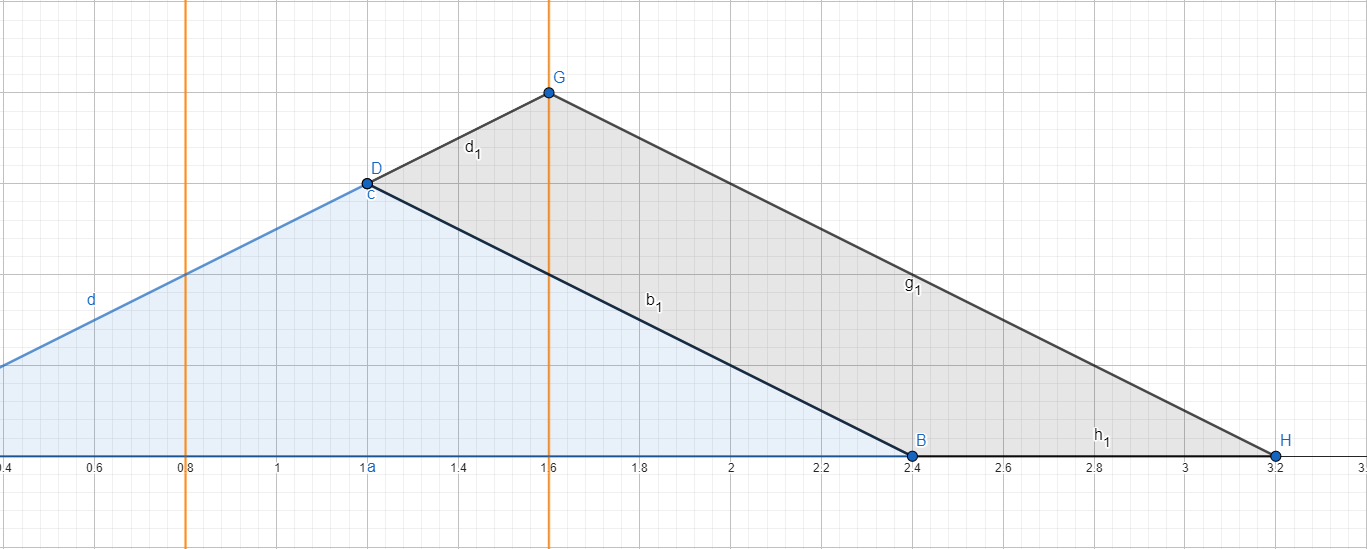
\includegraphics[scale=0.2]{img/interpolazione/compensateLateCallAccel1.png}
            \caption{CompensateLateCall quando acceleriamo}
            \label{fig:4_compensateLateCallAccel1}
        \end{figure}
    \end{minipage}

    \begin{minipage}{.475\textwidth}
        \[B = x\]
        \[H_t = \frac{a}{2}B\]
        \[A_t = \frac{BH_t}{2} = \frac{a}{4}x^2\]
        \[H_r = y\]
        \[A_r = BH_r = xy\]
    \end{minipage}
    \begin{minipage}{.475\textwidth}
        \begin{figure}[H]
            \centering
            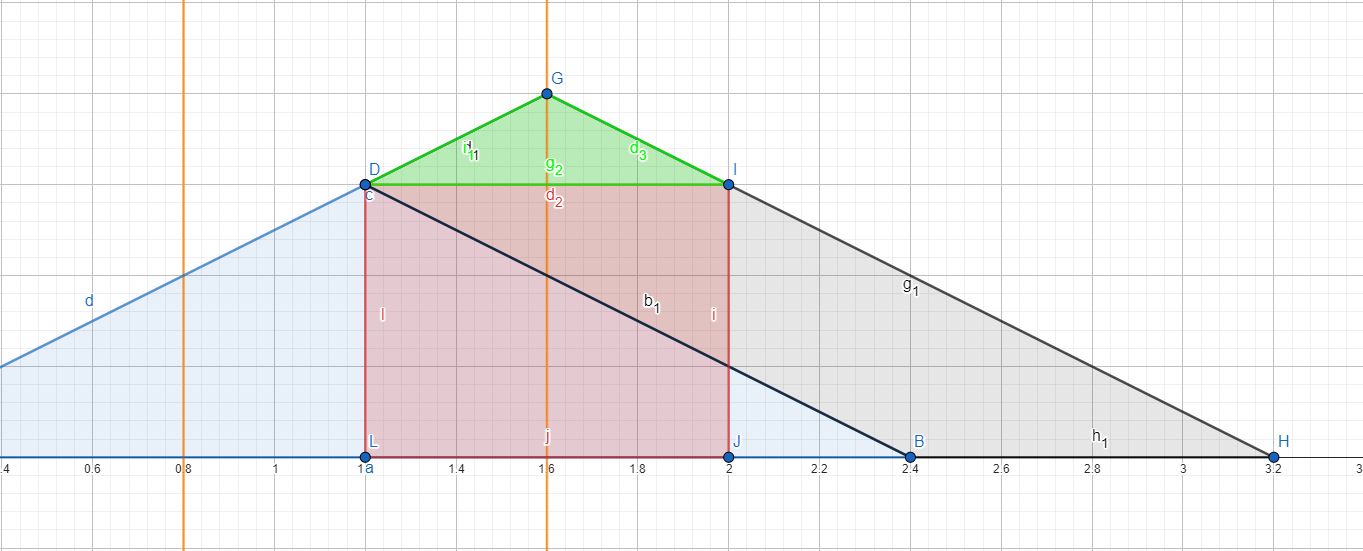
\includegraphics[width=1\linewidth]{img/interpolazione/compensateLateCallAccel2.png}
            \caption{Scomposizione del poligono quando stiamo accelerando}
            \label{fig:4_compensateLateCallAccel2}
        \end{figure}
    \end{minipage}
    
    Dove $a$ è uguale all'accelerazione. Riusciamo a calcolare l'altezza del triangolo a partire dall'accelerazione grazie al fatto che l'accelerazione rappresenta il rapporto tra la crescita della velocità rispetto al tempo impiegato.\newline
    Le formule per calcolarci l'area totale (corrispondente alla distanceDifference) e l'altezza totale (corrispondente alla velocità al tick corrente) sono:
    \hspace{2cm}
    
    \begin{minipage}{.45\textwidth}\[A = A_t + A_r = \frac{a}{4}x^2 + xy\]\end{minipage}
    \begin{minipage}{.45\textwidth}\[H = H_t + H_r = \frac{a}{4}x^2 + y\]\end{minipage}
    
    Mettendo queste due formule a sistema arriviamo ad ottenere la seguente equazione:
    \[\frac{a}{4}x^2 - Hx + A = 0\]
    Dove $A$, $H$ ed $a$ sono valori noti. Risolvendo l'equazione per x otteniamo quindi la base del nostro poligono, che corrisponde al doppio della differenza in secondi tra il tick corrente e quando avremmo dovuto iniziare a decelerare.
\end{itemize}

Una volta calcolato quanto tempo prima avremmo dovuto iniziare a decelerare, controlliamo se è un valore positivo. Se si, ricalcoliamo il movimento fino a quel momento e successivamente iniziamo a decelerare aggiornando il DeltaSeconds della funzione \lstinline{Update()} in modo che calcoli il resto dello spostamento.
Se invece il valore risulta negativo, vuol dire che TargetValue è cambiato tra questo ed il frame precedente. Questa casistica viene approfondita e gestita nel capitolo \say{Override Deceleration} \ref{subsubsec:4_2_OverrideDeceleration}.


\subsubsection{Override Deceleration}\label{subsubsec:4_2_OverrideDeceleration}
TargetValue potrebbe cambiare (avvicinandosi a CurrentValue) sia tra un frame e l'altro che mentre stiamo già decelerando. In tal caso è preferibile decelerare più in fretta piuttosto di fermarsi oltre TargetValue e poi tornare indietro (Vedi figura \ref{fig:4_OverrideDecelIntro}).
\begin{figure}[H]
    \centering
    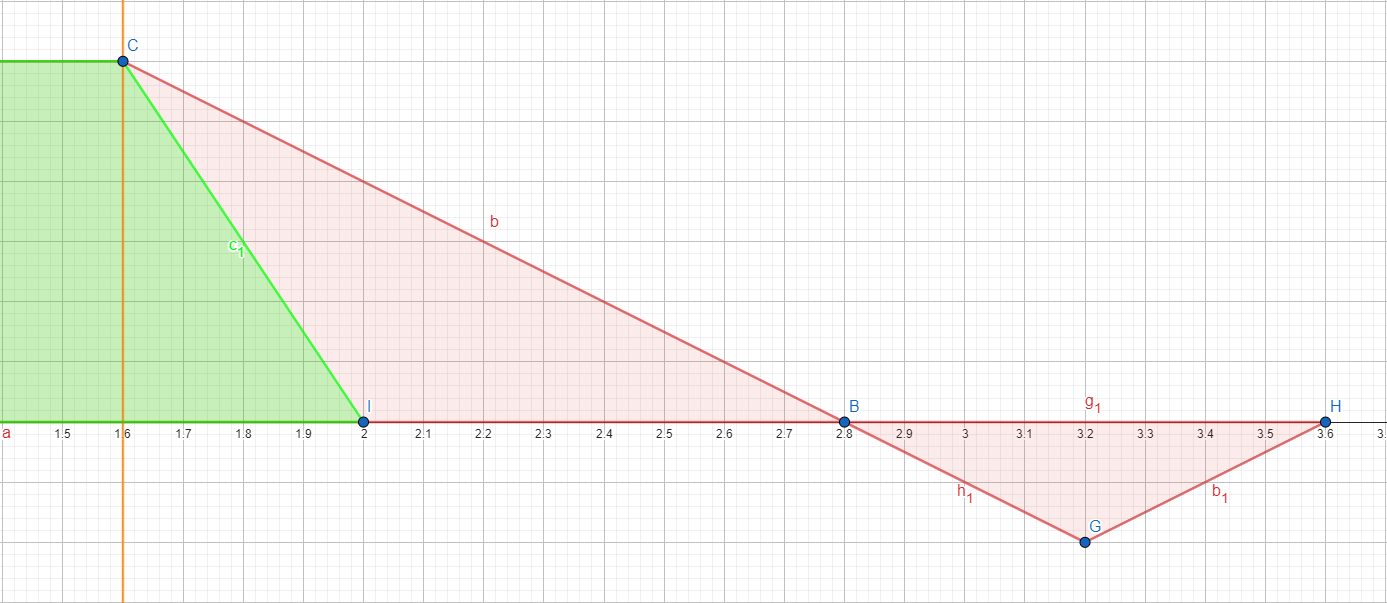
\includegraphics[width=.95\linewidth]{img/interpolazione/OverrideDecelIntro.png}
    \caption{Vogliamo che la nostra velocità si comporti come l'area verde, non come la rossa}
    \label{fig:4_OverrideDecelIntro}
\end{figure}
Questa correzione sulla decelerazione viene effettuata quando CompensateLateCall non è stata eseguita oppure ha fallito, stiamo decelerando, TargetValue è cambiato e la nostra stopPosition lo sorpassa. Queste condizioni fanno anche si che mentre stiamo già rallentando la decelerazione possa cambiare diventando sia più veloce che più lenta in base ai valori che vengono assegnati a TargetValue.
La differenza tra questa correzione e CompensateLateCall sta nel fatto che in quest'ultima il momento in cui avremmo dovuto iniziare a decelerare si trova tra il tick corrente ed il precedente, mentre in questo caso si trova prima del frame precedente. Poiché però non possiamo andare \say{indietro nel tempo} e correggere il calcolo effettuato dal tick precedente, l'unica scelta che abbiamo è quella di decelerare più in fretta.\newline

Poiché un motore non può fisicamente decelerare troppo in fretta, è presente un cap hard-coded alla massima velocità di decelerazione pari a $acceleration * 1.5$.

Per calcolarci il nuovo valore di decelerazione, ci serve sapere la stopDistance con una decelerazione normale e la velocità che avevamo nel frame precedente. Calcoliamo quindi la distanceDifference tra la stopDistance e TargetValue e eseguiamo l'operazione inversa per trovarci la base di un triangolo (timeDifference) a partire dalla sua area (distanceDifference) e la sua altezza (prevSpeed). Sottraendo timeDifference a DeltaSeconds ci troviamo il tempo in secondi (Punto $G$ nella figura \ref{fig:4_OverrideDecelTimeDiff}) che impiegheremo per raggiungere TargetValue con una velocità che decresce linearmente.
\[stopTime = DeltaSeconds - \frac{distanceDifference * 2}{prevSpeed}\]
\begin{figure}[H]
    \centering
    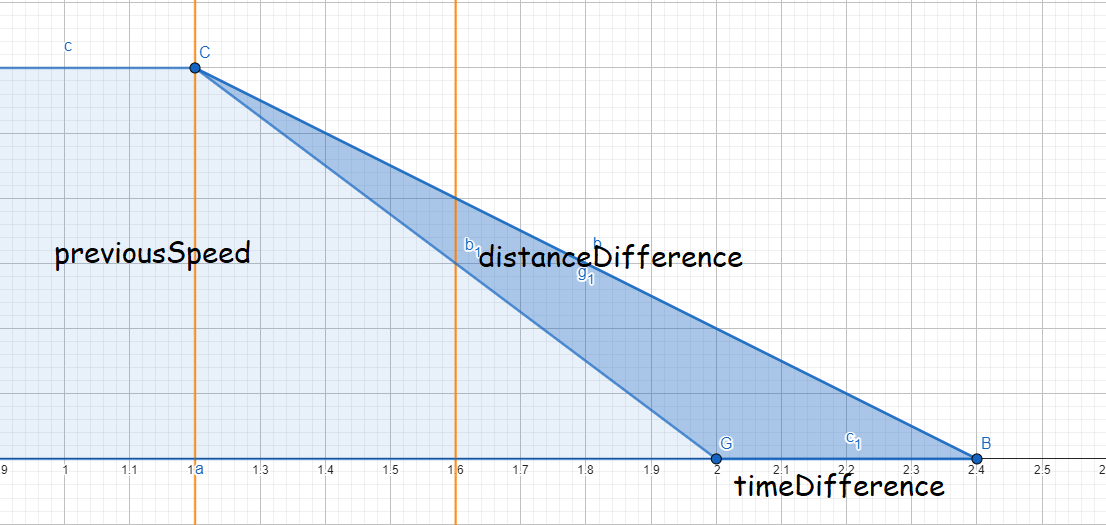
\includegraphics[width=.95\linewidth]{img/interpolazione/OverrideDecelTimeDiff.png}
    \caption{Il punto $G$ è il momento in cui la nostra toccherà lo zero raggiungendo TargetValue}
    \label{fig:4_OverrideDecelTimeDiff}
\end{figure}
Il valore di decelerazione corrisponde al coefficiente della retta passante tra il punto in cui iniziamo a decelerare ($C$) e $G$. Assumiamo quindi che $C$ abbia la coordinata X pari a 0. $C$ si troverà quindi a (0, prevSpeed), mentre $G$ si troverà a (stopTime, 0). Possiamo trovato il coefficiente di questa retta usando la formula:
\[\frac{y_2 - y_1}{x_2 - x_1}\]
Che, nel nostro caso, corrisponde a:
\[acceleration = \frac{0 - prevSpeed}{stopTime - 0} = -\frac{prevSpeed}{stopTime}\]

Una volta trovato questo valore, il codice farà un rollback al tick precedente e ricalcolerà lo spostamento (così come i prossimi) con il nuovo valore di accelerazione.
\clearpage %TODO CONTROLLARE SE SERVE ANCORA

\subsubsection{SpeedCap per i piccoli movimenti}\label{subsubsec:4_2_Speedcap}
%TODO

\subsubsection{Conversioni da RealFade e RealAcceleration}\label{subsubsec:4_2_Conversions}
%TODO

\end{document}